\documentclass[format=sigconf, review=false, screen=true]{acmart}

\usepackage{booktabs} % For formal tables

% Metadata Information
%\acmJournal{FAT*}
\acmVolume{}
\acmNumber{}
\acmArticle{}
\acmYear{2019}
\acmMonth{9}
\copyrightyear{2019}
%\acmArticleSeq{9}
\acmConference[Preprint in Review]{ArXiV Computing Research Repository}{}

% DOI
\acmDOI{}

% Paper history
\received{April 2019}
\received[revised]{July 2019}
\received[revised]{August 2019}
%\received[accepted]{June 2009}


% Copyright
%\setcopyright{acmcopyright}
\setcopyright{acmlicensed}
%\setcopyright{rightsretained}
%\setcopyright{usgov}
%\setcopyright{usgovmixed}
%\setcopyright{cagov}
%\setcopyright{cagovmixed}

\usepackage[ruled]{algorithm2e} % For algorithms
\renewcommand{\algorithmcfname}{ALGORITHM}
\SetAlFnt{\small}
\SetAlCapFnt{\small}
\SetAlCapNameFnt{\small}
\SetAlCapHSkip{0pt}
\IncMargin{-\parindent}
% Arabic page numbers for submission.  Remove this line to eliminate
% page numbers for the camera ready copy
% \pagenumbering{arabic}

% Load basic packages
\usepackage{balance}       % to better equalize the last page
\usepackage{graphics}      % for EPS, load graphicx instead
\usepackage{todonotes}     % for \todo
%\usepackage[T1]{fontenc}   % for umlauts and other diaeresis
%\usepackage{txfonts}
%\usepackage{mathptmx}
%\usepackage[pdflang={en-US},pdftex]{hyperref}
%\usepackage{color}
\usepackage{booktabs}
\usepackage{subcaption}
\usepackage{textcomp}
\PassOptionsToPackage{warn}{textcomp}
%\usepackage[table]{xcolor}

% Some optional stuff you might like/need.
\usepackage{microtype}        % Improved Tracking and Kerning
% \usepackage[all]{hypcap}    % Fixes bug in hyperref caption linking
% \usepackage{ccicons}          % Cite your images correctly!
% \usepackage[utf8]{inputenc} % for a UTF8 editor only

% If you want to use todo notes, marginpars etc. during creation of
% your draft document, you have to enable the "chi_draft" option for
% the document class. To do this, change the very first line to:
% "\documentclass[chi_draft]{sigchi}". You can then place todo notes
% by using the "\todo{...}"  command. Make sure to disable the draft
% option again before submitting your final document.
%\usepackage{todonotes}

% Paper metadata (use plain text, for PDF inclusion and later
% re-using, if desired).  Use \emtpyauthor when submitting for review
% so you remain anonymous.


\newcommand{\FIXME}[1]{\textcolor{red}{[\textbf{FIXME}: \textit{#1}]}}
\newcommand{\TODO}[1]{\textcolor{red}{[\textbf{FIXME}: \textit{#1}]}}

\newcommand\leadin[1]{%
    \vskip 5pt \noindent\textbf{#1.} %
}
\newcommand\leadinx[1]{%
    \vskip 5pt \noindent\textbf{#1} %
}

%
%\def\sharedaffiliation{%
%\end{tabular}
%\begin{tabular}{c}}
%

\clubpenalty=10000
\widowpenalty=10000

% llt: Define a global style for URLs, rather that the default one
%\makeatletter
%\def\url@leostyle{%
%  \@ifundefined{selectfont}{
%    \def\UrlFont{\sf}
%  }{
%    \def\UrlFont{\small\bf\ttfamily}
%  }}
%\makeatother
%\urlstyle{leo}

% To make various LaTeX processors do the right thing with page size.
%\def\pprw{8.5in}
%\def\pprh{11in}
%\special{papersize=\pprw,\pprh}
%\setlength{\paperwidth}{\pprw}
%\setlength{\paperheight}{\pprh}
%\setlength{\pdfpagewidth}{\pprw}
%\setlength{\pdfpageheight}{\pprh}

% Make sure hyperref comes last of your loaded packages, to give it a
% fighting chance of not being over-written, since its job is to
% redefine many LaTeX commands.
% \definecolor{linkColor}{RGB}{6,125,233}

% create a shortcut to typeset table headings
% \newcommand\tabhead[1]{\small\textbf{#1}}


% Document starts
\begin{document}

% Title portion. Note the short title for running heads
\title[ORES]{ORES: Lowering Barriers with Participatory Machine Learning in Wikipedia}

\author{Redacted F. Review}
\orcid{1234-5678-9012-3456}
\affiliation{%
  \institution{XXXXXXX}
  \streetaddress{XXXXXXX}
  \city{XXXXX}
  \state{XX}
  \postcode{12345}
  \country{XXX}}
\email{XXXX@XX.XX}

\author{Redacted G. Review}
\orcid{1234-5678-9012-3456}
\affiliation{%
  \institution{XXXXXXX}
  \streetaddress{XXXXXXX}
  \city{XXXXX}
  \state{XX}
  \postcode{12345}
  \country{XXX}}
\email{XXXX@XX.XX}

\renewcommand{\shortauthors}{XXX et al.}


\begin{abstract}
Algorithmic systems---from rule-based bots to machine learning classifiers---have a long history of supporting the essential work of content moderation and other curation work in peer production projects.  From counter-vandalism to task routing, basic machine prediction has allowed open knowledge projects like Wikipedia to scale to the largest encyclopedia in the world, while maintaining quality and consistency.  However, conversations about how quality control should work and what role algorithms should play have generally been led by the expert engineers who have the skills and resources to develop and modify these complex algorithmic systems. In this paper, we describe ORES: an algorithmic scoring service that supports real-time scoring of wiki edits using multiple independent classifiers trained on different datasets. ORES decouples several activities that have typically all been performed by engineers: choosing or curating training data, building models to serve predictions, auditing predictions, and developing interfaces or automated agents that act on those predictions. This meta-algorithmic system was designed to open up socio-technical conversations about algorithmic systems in Wikipedia to a broader set of participants.  In this paper, we discuss the theoretical mechanisms of social change ORES enables and detail case studies in participatory machine learning around ORES from the 4 years since its deployment.

\end{abstract}


% %
% The code below should be generated by the tool at
% http://dl.acm.org/ccs.cfm
% Please copy and paste the code instead of the example below.
%
\begin{CCSXML}
<ccs2012>
<concept>
<concept_id>10003033.10003106.10003114.10011730</concept_id>
<concept_desc>Networks~Online social networks</concept_desc>
<concept_significance>500</concept_significance>
</concept>
<concept>
<concept_id>10010147.10010257.10010258.10010259.10010263</concept_id>
<concept_desc>Computing methodologies~Supervised learning by classification</concept_desc>
<concept_significance>500</concept_significance>
</concept>
<concept>
<concept_id>10010405.10010455.10010461</concept_id>
<concept_desc>Applied computing~Sociology</concept_desc>
<concept_significance>500</concept_significance>
</concept>
<concept>
<concept_id>10011007.10011074.10011075.10011079.10011080</concept_id>
<concept_desc>Software and its engineering~Software design techniques</concept_desc>
<concept_significance>500</concept_significance>
</concept>
<concept>
<concept_id>10010520.10010521.10010537.10003100</concept_id>
<concept_desc>Computer systems organization~Cloud computing</concept_desc>
<concept_significance>100</concept_significance>
</concept>
</ccs2012>
\end{CCSXML}


\ccsdesc[500]{Networks~Online social networks}
\ccsdesc[500]{Computing methodologies~Supervised learning by classification}
\ccsdesc[500]{Applied computing~Sociology}
\ccsdesc[500]{Software and its engineering~Software design techniques}
\ccsdesc[100]{Computer systems organization~Cloud computing}

%
% End generated code
%



%
% End generated code
%


\keywords{Wikipedia, Reflection, Machine learning, Transparency, Fairness, Algorithms, Governance}
\settopmatter{printfolios=true}
\maketitle

\section{Introduction}
\label{sec:introduction}
Wikipedia---the free encyclopedia that anyone can edit---faces many challenges in maintaining the quality of its articles and sustaining the volunteer community of editors. The people behind the hundreds of different language versions of Wikipedia have long relied on automation, bots, expert systems, recommender systems, human-in-the-loop assisted tools, and machine learning to help moderate and manage content at massive scales. The issues around artificial intelligence in Wikipedia are as complex as those facing other large-scale user-generated content platforms like Facebook, Twitter, or YouTube, as well as traditional corporate and governmental organizations that must make and manage decisions at scale. And like in those organizations, Wikipedia's automated classifiers are raising new and old issues about truth, power, responsibility, openness, and representation.

Yet Wikipedia's approach to AI has long been different than in corporate or governmental contexts typically discussed in emerging fields like Fairness, Accountability, and Transparency in Machine Learning (FATML) or Critical Algorithms Studies (CAS). The volunteer community of editors has strong ideological principles of openness, decentralization, and consensus-based decision-making. The paid staff at the non-profit Wikimedia Foundation---which legally owns and operates the servers---are not tasked with making editorial decisions about content\footnote{Except in rare cases, such as content that violates U.S. law, see \url{http://enwp.org/WP:OFFICE}}. This is instead the responsibility of the volunteer community, where a self-selected set of developers build tools, bots, and advanced technologies in broad consultation with the community. Even though Wikipedia's longstanding socio-technical system of algorithmic governance is far more open, transparent, and accountable than most platforms operating at Wikipedia's scale, ORES\footnote{\url{https://ores.wikimedia.org} and \url{http://enwp.org/:mw:ORES}}, the system we present in this paper, pushes even further on the crucial issue of who is able to participate in the development and use of advanced technologies.

ORES represents several innovations in openness in machine learning, particularly in seeing openness as a socio-technical challenge that is as much about scaffolding support as it is about open-sourcing code and data. With ORES, volunteers can curate labeled training data from a variety of sources for a particular purpose, commission the production of a machine classifier based on particular approaches and parameters, and make this classifier available via an API which anyone can query to score any edit to a page---operating in real time on the Wikimedia Foundation's servers. Currently, 102 classifiers have been produced for 41 languages, classifying edits in real-time based on criteria like ``damaging / not damaging,'' ``good faith / bad faith,'' or a language-specific article quality scale. ORES intentionally does not seek to produce a single classifier to enforce a gold standard of quality, nor does it prescribe particular ways in which scores and classifications will be incorporated into fully automated bots and semi-automated editing interfaces. As we will describe in section~\ref{sec:design_rationale}, ORES was built as a kind of cultural probe \cite{hutchinson2003technology} to support an open-ended set of community efforts to re-imagine what machine learning in Wikipedia is and who it is for.

Open participation in machine learning is widely relevant to both researchers of user-generated content platforms and those working across open collaboration, social computing, machine learning, and critical algorithms studies. ORES implements several of the dominant recommendations for algorithmic system builders around transparency and community consent\cite{crawford2016algorithm,diakopoulos2015algorithmic,sandvig2014auditing}. We discuss practical scoio-technical considerations for what openness, accountability, and transparency mean in a large-scale, real-world user-generated content platform. Wikipedia is also an excellent space for work on FATML topics, as the broader Wikimedia community and the non-profit Wikimedia Foundation are founded on ideals of open, public participation. All of the work presented in this paper is publicly-accessible and open sourced, from the source code and training data to the community discussions about ORES. Unlike in other nominally `public` platforms where users often do not know their data is used for research purposes, Wikipedians have extensive discussions about using their archived activity for research, with established guidelines we followed.\footnote{See \url{http://enwp.org/WP:NOTLAB} and \url{http://enwp.org/WP:Ethically_researching_Wikipedia}} This project is part of a longstanding engagement with the volunteer communities which involves extensive community consultation, and the case studies research have been approved by a university IRB.

In this paper, we first review related literature around open algorithmic systems, then discuss the socio-technical context of Wikipedia that lead us to building ORES. We discuss the operation of ORES, highlighting innovations in algorithmic \emph{openness} and \emph{transparency}. We present case studies of ORES that illustrate how it has broadened participation in machine learning.  Finally, we conclude with a discussion of the issues raised by this work and identify future directions.


\section{Related work}
\label{sec:related_work}
\subsection{The politics of algorithms}
Algorithmic systems play increasingly crucial roles in the governance of social processes \cite{gillespie2014relevance}. Software algorithms are increasingly used in answering questions that have no single right answer and where using prior human decisions as training data can be problematic \cite{barocas2013governing}. Algorithms designed to support work change people's work practices, shifting how, where, and by whom work is accomplished \cite{crawford2016algorithm, zuboff1988age}. Software algorithms gain political relevance on par with other process-mediating artifacts (e.g. laws, norms \cite{lessig1999code}).

There are repeated calls to address power dynamics and bias through transparency and accountability of the algorithms that govern public life and access to resources \cite{diakopoulos2017algorithmic,sandvig2014auditing}. The field around effective transparency, explainability, and accountability mechanisms is growing. We cannot fully address the scale of concerns in this rapidly shifting literature, but we find inspiration in Kroll et al's discussion of the limitations of auditing and transparency \cite{kroll2016accountable}, Mulligan et al's shift towards the term ``contestability'' \cite{mulligan2019shaping}, and Geiger's call to go ``beyond opening up the black box\cite{geiger2017beyond}''.

In this paper, we discuss a specific socio-political context---Wikipedia's algorithmic quality control and socialization practices---and the development of novel algorithmic systems for support of these processes.  We implement a meta-algorithmic intervention aligned with Wikipedians' principles and practices: deploying a set of prediction algorithms as a service and leaving decisions about appropriation to the volunteer community.  Instead of training the single best classifier and implementing it in our own designs, we embrace public auditing, re-interpretations, and appropriations of our models' predictions as an \emph{intended} and \emph{desired} outcome.  Extensive work on technical and social ways to achieve fairness and accountability generally do not discuss this kind of socio-infrastructural intervention on communities of practice.

\subsection{Machine prediction in support of open production}
Open peer production systems, like all user-generated content platforms, have a long history of using machine learning for content moderation and task management. For Wikipedia and related Wikimedia projects, vandalism detection and quality control is a major goal for practitioners and researchers.  Article quality prediction models have also been explored and applied to help Wikipedians focus their work in the most beneficial places.

\leadin{Vandalism detection} The damage detection problem in Wikipedia is one of great scale.  English Wikipedia receives about 160,000 new edits every day, which immediately go live without review.  Wikipedians embrace this risk as the nature of an open encyclopedia, but work tirelessly to maintain quality. Every damaging or offensive edit puts the credibility of the community and their product at risk, so all edits must be reviewed as soon as possible \cite{geiger2010work}. As an information overload problem, filtering strategies using machine learning models have been developed to support the work of Wikipedia's patrollers (see \cite{adler2011wikipedia} for an overview).  In some cases, researchers directly integrated their prediction models into purpose-designed tools for Wikipedians to use (e.g. STiki \cite{west2010stiki}, a classifier-supported human-computation tool). Through these machine learning models and constant patrolling, most damaging edits are reverted within seconds of when they are saved \cite{geiger2013levee}.

\leadin{Task routing and recommendation}
Machine learning plays a major role in how Wikipedians decide what articles to work on, supplementing the standard self-selected dynamic of people contributing to topics they are interested in. Wikipedia has many well-known content coverage biases (e.g. for a long period of time, the coverage of women scientists in Wikipedia lagged far behind the rest of the encyclopedia \cite{halfaker2017interpolating}). Past work has explored collaborative recommender-based task routing strategies (see SuggestBot \cite{cosley2007suggestbot}), in which contributors are sent articles that need improvement in their areas of expertise. Such systems show strong promise to address content coverage biases, but could also inadvertently reinforce biases.

\subsection{The Rise and Decline: Wikipedia's socio-technical problems}
While Wikipedians have successfully deployed algorithmic quality control support systems to maintain Wikipedia, a line of critical research has studied the unintended consequences of this complex socio-technical system, particularly on newcomer socialization~\cite{halfaker2013rise,morgan2013tea,halfaker2014snuggle}.  In summary, Wikipedians struggled with the issues of scaling when the popularity of Wikipedia grew exponentially between 2005 and 2007~\cite{halfaker2013rise}.  In response, they developed quality control processes and technologies that prioritized efficiency by using machine prediction models~\cite{halfaker2014snuggle} and templated warning messages~ \cite{halfaker2013rise}.  This transformed newcomer socialization from a primarily human and welcoming activity to one that is more dismissive and impersonal~\cite{morgan2013tea} and has caused in a steady decline in Wikipedia's editing population.  The efficiency of quality control work and the elimination of damage was considered extremely politically important, while the positive experience of newcomers was less so. After the research about this systemic issue came out, the political importance of newcomer experience was raised substantially.  But despite targeted efforts and shifts in perception among some members of the Wikipedia community~\cite{narayan2015effects, morgan2013tea}\footnote{See also a team dedicated to supporting newcomers\url{http://enwp.org/:m:Growth team}}, the quality control processes that were designed over a decade ago remain largely unchanged~\cite{halfaker2014snuggle}.

Wikipedian tool developers play a critical role in the larger conversation of how the community should be doing quality control~\cite{geiger2014bots, halfaker2014snuggle}. There are few formal barriers to anyone auditing, modifying, or developing their own classifier: there is substantial transparency both in open licensing of code and data, as well as an open and public governance model. However, Wikipedia's massive scale means that significant computational and data engineering expertise are required do so. This limits the types of people who are able to participate in the technological side of such a conversation.  Historically, tool developers who were motivated and capable of developing such tools chose to optimize for efficiency to the exclusion of other goals~\cite{halfaker2014snuggle}.  Today, we know that many of these other goals --- especially those related to newcomer retention and the diversity of contributors\footnote{\url{https://meta.wikimedia.org/wiki/Strategy/Wikimedia_movement/2017/Direction}} --- are also important~\cite{morgan2013tea, halfaker2013rise}.  In this paper, we describe a system that is designed to open up the technical side of this quality control conversation. Our aim is to allow a more diverse set of values to be represented, and for these values of the broader community to be more coherently expressed.

\section{Design rationale}
\label{sec:design_rationale}
In this section, we discuss systemic mechanisms behind Wikipedia's socio-technical problems and how we as system builders designed ORES to have impact within Wikipedia.  Past work has demonstrated how Wikipedia's problems are systemic and caused in part to inherent biases in the system of quality control. To responsibly use machine learning in addressing these problems, we examined how Wikipedia functions as a distributed system, focusing on how processes, policies, power, and software come together to make Wikipedia happen.

\subsection{The problem: Stagnation in quality control practices}
As discussed in the previous section, while there is an apparent need for re-engineering Wikipedia's quality control practices and many efforts to make improvements, the quality control processes that were designed over a decade ago remain largely unchanged~\cite{halfaker2014snuggle}.  Why is this work practice so hard to make adjustments to?

Like the rest of Wikipedia's system of processes, quality control policy and practice are open to redesign via a consensus\footnote{\url{https://enwp.org/WP:CONSENSUS}} conversation.  Historically, the people with the skills and inclination to develop software tools that support work processes in Wikipedia have held a large amount of power in deciding what types of work will and will not be supported~\cite{niederer2010wisdom,geiger2011lives,muller2013work,tkacz2014wikipedia,livingstone2016population}.  In theory, one promising strategy to change quality control practices is to develop tools that capture an alternative vision of what's important (e.g. focusing on newcomer socialization or supporting a diverse set of newcomers).  

However, building a software system that would be useful for quality control work for Wikipedia is very difficult.  Scale and efficiency are critical considerations in the work practice of quality control in Wikipedia.  English Wikipedia sees over 142K edits per day\footnote{\url{https://quarry.wmflabs.org/query/38370}}.  If a reviewer could check 1 revision every 5 seconds, it would require 192 labor hours \emph{per day} to check all edits for blatant vandalism, hoaxes, and mistakes --- and this rate would only involve a cursory check.  The consequences of not dealing with damaging edits quickly and efficiently are quite high.  For example, losing just one of the components of the current complex regime of counter-vandalism tools has resulted in periods of Wikipedia's history where vandalism gathered twice as many views on average before being reverted~\cite{geiger2013levee}.

Without exception, all of the critical, efficient quality control tools that help keep Wikipedia clean of vandalism and other damage employ a real-time machine prediction model for flagging the edits that are most likely to be damaging. For example, Huggle and STiki\footnote{\url{http://enwp.org/WP:STiki}} use machine prediction models to highlight likely damaging edits for human review, and ClueBot NG\footnote{\url{http://enwp.org/User:ClueBot_NG}} uses a machine prediction model to automatically revert edits that are highly likely to be damaging.  All of these tools were first developed during the exponential growth period in Wikipedia's history --- before the social issues in quality control dynamics were apparent~\cite{halfaker2013rise}. Despite recent work to improve support for newcomers, these same tools and the processes they support continue to remain dominant today.  

\subsection{Our goal: Lowered barriers to participation}
For anyone looking to enact a new view of quality control into the designs of a software tool, there is a high barrier to entry: they must have the technical competency to design, build and manage a real-time, multilingual machine classifier that operates at Wikipedia's scale.  This is a narrow set of technical skills and capacities that few of the volunteers in the Wikipedian community possess.  Even those with advanced skills in machine learning and data engineering often have day jobs that prevent them from investing the time necessary to maintain these systems~\cite{sculley2015hidden}. Given Wikipedia's open participation model but continual issues with diversity and inclusion, it is important to note that free time is not equitably distributed in society~\citep{Bianchi2010}. 

In past work, researchers sought to directly enact alternative visions of quality control in Wikipedian tools by developing new alternatives premised on different values~\cite{halfaker2014snuggle}. However, these have generally not been adopted, and so we see more potential in employing a margin-building strategy --- akin to Nelle Morten's concept of ``hearing to speech''\footnote{Here we were inspired by Bowker and Star's reference to Nelle's work in their seminal book "Sorting Things Out"\cite{bowker1999sorting}}\cite{morton1985journey}: ``Speaking first to be heard is power over. Hearing to bring forth speech is empowering.''  While past work sought to ``speak'' about how quality control should be, we seek to employ a different tactic: broaden the diversity of voices participating in the \emph{conversation} about quality control practices by enabling more people to experiment with designing, auditing, redesigning, and implementing automated tools. 

Through the development of ORES, we explore the possibility of expanding the margins of this conversation\cite{mugar2017preserving}.  We think that deploying a high-availability machine prediction service, designing accessible interfaces, and engaging in basic outreach efforts, we will be able to dramatically lower the barriers to the development of new algorithmic tools that could implement new ideas about what should be classified, how it should be classified, and how classifications and scores should be used.  

\subsection{Our measure of success: More voices}
Our goal in this intervention is to ``hear to speech'': to enable those who were not able to participate in the \emph{socio-technical} conversation about Wikipedia's quality control practices to more easily have a voice.  So unlike most machine learning projects, we measure success not through higher rates of precision and recall (though we are, of course, interested in that as well), but instead though the new conversations about how algorithmic tools affect editing dynamics.  If ORES is a successful intervention, it will enable experimentation in Wikipedia's socio-technical \emph{conversations} about quality control.  This translates into the development of novel tools and serious, critical reflection on the roles that algorithms play in mediating Wikipedia's quality and newcomer support processes. If we only see the same discussions (e.g. "How do we make vandal fighting more efficient?") and similar tools focused on quality control to the exclusion of newcomer socialization, we will know that we have missed the mark.

\section{The ORES system}
\label{sec:the_ores_system}
\begin{figure*}[h!]
  \centering
  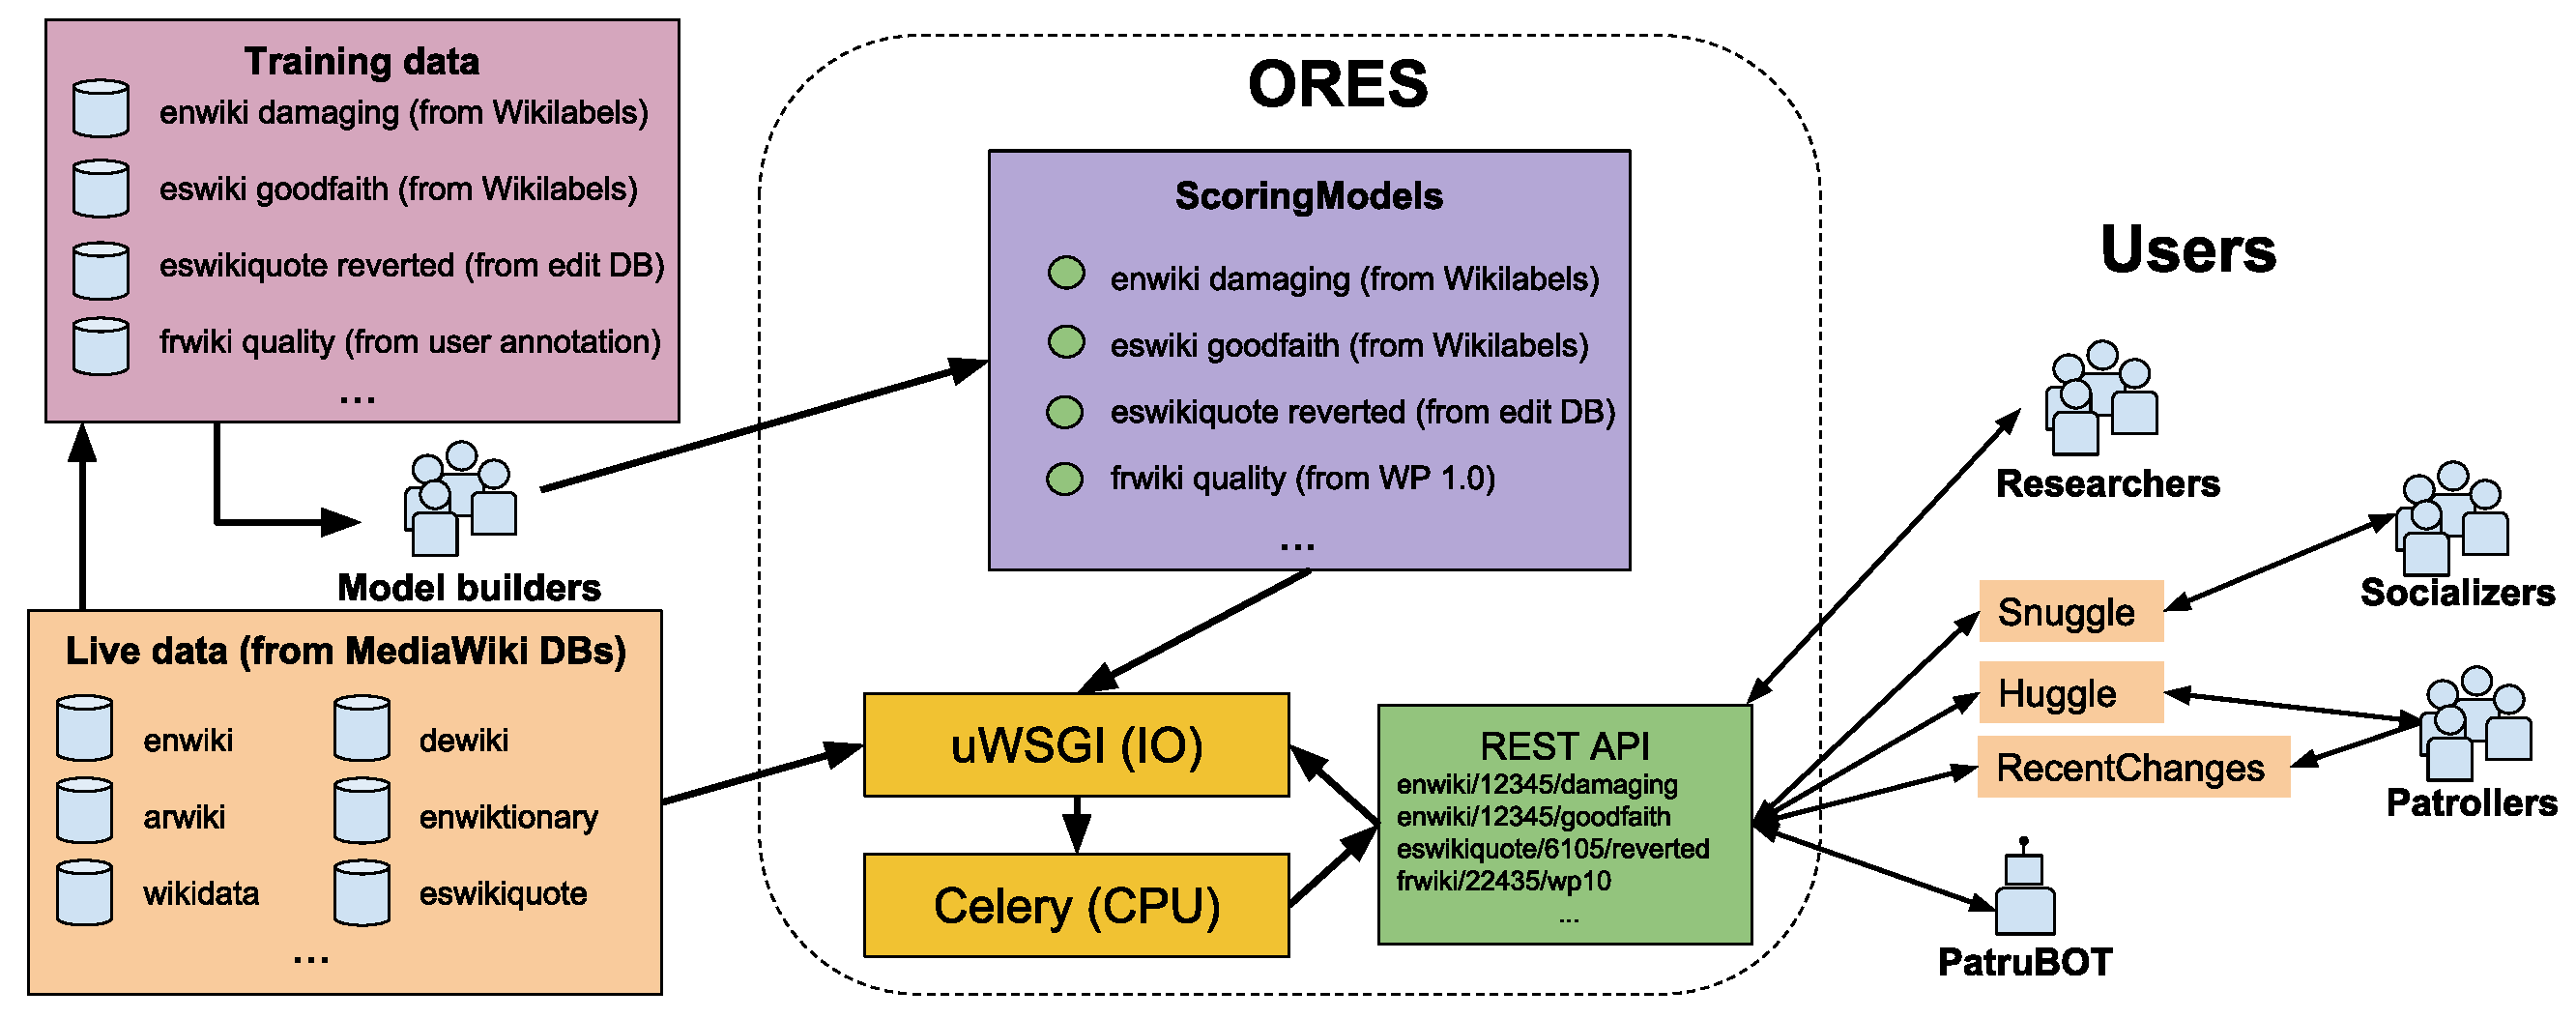
\includegraphics[width=.95\textwidth]{figures/ores_data_user_diagram}
  \caption{ORES conceptual overview.  Model builders design process for training ScoringModels from training data.  ORES hosts ScoringModels and makes them available to researchers and tool developers.}
  \label{fig:ores_data_user}
\end{figure*}

ORES has been iteratively engineered to meet the needs of Wikipedia editors and the tools that support their work (see section~\ref{sec:ores_system_engineering}). It is a machine learning as a service platform that enables Wikipedians and researchers to commission a new classifier, which are hosted by the Wikimedia Foundation for anyone to query. Figure  \ref{fig:ores_data_user} gives a conceptual overview, showing how ORES is a collection of machine classifier models and an web-based API, which connect to various sources of training data (to build the models) and live data (to apply the models). These models are designed and engineered by a varied set of model builders, some are external researchers and others are our own engineering team.  The models that ORES hosts are based on quite different sets of curated training data and have been engineered to support Wikipedian processes related to damage-detection, quality-assessment, and topic-routing. In general, the system is adaptable to a wide range of other models.

To make these models available for users, ORES implements a simple container service where the ``container,'' referred to as a \emph{ScoringModel}, represents a fully trained and tested prediction model.  All \emph{ScoringModels} contain metadata about when the model was train/tested and code for feature extraction.  All predictions take the form of a JSON document.  The ORES service provides access to ScoringModels via a RESTful HTTP interface and serves the predictions to users (see Figure~\ref{fig:english_wp10_prediction} for an example score request).  We chose this service structure because Wikimedian tool developers (our target audience) are familiar with this RESTful API/JSON workflow due to the dominant use of the MediaWiki API among tool developers.

\subsection{Score documents}
\label{sec:appendix.score_documents}
The predictions made by ORES are human- and machine-readable.  In general, our classifiers will report a specific prediction along with a set of probability (likelihood) for each class.  By providing detailed information about a prediction, we allow users to re-purpose the prediction for their on use.  Consider article quality (wp10) prediction output in Figure~\ref{fig:english_wp10_prediction}.

\begin{figure}[h!]
        \makebox{\hrulefill}{
        \small
        \begin{verbatim}
"wp10": {
  "score": {
    "prediction": "Start",
    "probability": {
      "FA": 0.00329313015, "GA": 0.0058529554,
      "B": 0.06062338048, "C": 0.01991363271,
      "Start": 0.754330134, "Stub": 0.1559867667
    }
  }
}
        \end{verbatim}
        \hrule
        \normalsize}
        \caption{Result of \url{https://ores.wikimedia.org/v3/scores/enwiki/34234210/wp10}}
        \label{fig:english_wp10_prediction}
\end{figure}

A developer making use of a prediction like this may choose to present the raw prediction ``Start'' (one of the lower quality classes) to users or to implement some visualization of the probability distribution across predicted classed (75\% Start, 16\% Stub, etc.).  They might even choose to build an aggregate metric that weights the quality classes by their prediction weight (e.g. Ross's student support interface\cite{ross2016visualizing} or the \emph{weighted sum} metric from~\cite{halfaker2017interpolating}).

\subsection{Model information}
\label{sec:appendix.model_information}
In order to use a model effectively in practice, a user needs to know what to expect from model performance.  E.g. how often is it that when an edit is predicted to be ``damaging'' it actually is? (\emph{precision}) or what proportion of damaging edits should I expect will be caught by the model? (\emph{recall})  The target metric of an operational concern depends strongly on the intended use of the model.  Given that our goal with ORES is to allow people to experiment with the use and reflection of prediction models in novel ways, we sought to build an general model information strategy.

\begin{figure}[htbp]
        \makebox{\hrulefill}{
        \small
        \begin{verbatim}
"damaging": {
  "type": "GradientBoosting",
  "version": "0.4.0",
  "environment": {"machine": "x86_64", ...},
  "params": {"center": true, "init": null,
             "label_weights": {"true": 10},
             "labels": [true, false],
             "learning_rate": 0.01,
             "min_samples_leaf": 1,
             ...},
  "statistics": {
    "counts": {
      "labels": {"false": 18702, "true": 743},
      "n": 19445,
      "predictions": {
        "false": {"false": 17989, "true": 713},
        "true": {"false": 331, "true": 412}}},
    "precision": {
      "labels": {"false": 0.984, "true": 0.34},
      "macro": 0.662, "micro": 0.962},
    "recall": {
      "labels": {"false": 0.962, "true": 0.555},
      "macro": 0.758, "micro": 0.948},
    "pr_auc": {
      "labels": {"false": 0.997, "true": 0.445},
      "macro": 0.721, "micro": 0.978},
    "roc_auc": {
      "labels": {"false": 0.923, "true": 0.923},
      "macro": 0.923, "micro": 0.923},
    ...
  }
}
        \end{verbatim}
        \hrule
        \normalsize}
        \caption{Result of \url{https://ores.wikimedia.org/v3/scores/enwiki/?model_info&models=damaging}}
        \label{fig:english_damaging_model_info}
\end{figure}

The output captured in Figure~\ref{fig:english_damaging_model_info} shows a heavily trimmed JSON (human- and machine-readable) output of \emph{model\_info} for the ``damaging'' model in English Wikipedia.  Note that many fields have been trimmed in the interest of space with an ellipsis (``...'').  What remains gives a taste of what information is available.  Specifically, there is structured data about what kind of model is being used, how it is parameterized, the computing environment used for training, the size of the train/test set, the basic set of fitness metrics, and a version number so that secondary caches know when to invalidate old scores.  A developer using an ORES model in their tools can use these fitness metrics to make decisions about whether or not a model is appropriate and to report to users what fitness they might expect at a given confidence threshold.

\subsection{Threshold optimization}
\label{sec:appendix.threshold_optimization}
When we first started developing ORES, we realized that operational concerns of Wikipedia's curators need to be translated into confidence thresholds for the prediction models.  For example, counter-vandalism patrollers seek to catch all (or almost all) vandalism before it stays in Wikipedia for very long.  That means they have an operational concern around the \emph{recall} of a damage prediction model.  They would also like to review as few edits as possible in order to catch that vandalism.  So they have an operational concern around the \emph{filter rate}---the proportion of edits that are not flagged for review by the model\cite{halfaker2016notes}.

By finding the threshold of prediction likelihood that optimizes the filter-rate at a high level of recall, we can provide vandal-fighters with an effective trade-off for supporting their work.  We refer to these optimizations in ORES as \emph{threshold optimizations} and ORES provides information about these thresholds in a machine-readable format so that tools can automatically detect the relevant thresholds for their wiki/model context.

Originally, when we developed ORES, we defined these threshold optimizations in our deployment configuration.  But eventually, it became apparent that our users wanted to be able to search through fitness metrics to choose thresholds that matched their own operational concerns.  Adding new optimizations and redeploying quickly became a burden on us and a delay for our users.  In response, we developed a syntax for requesting an optimization from ORES in real-time using fitness statistics from the models tests. E.g. \texttt{maximum recall @ precision >= 0.9} gets a useful threshold for a counter-vandalism bot or \texttt{maximum filter\_rate @ recall >= 0.75} gets a useful threshold for semi-automated edit review (with human judgement).

\begin{figure}[htbp]
        \makebox{\hrulefill}{
        \small
        \begin{verbatim}
  {"threshold": 0.30, ...,
   "filter_rate": 0.88, "fpr": 0.097,
   "precision": 0.21, "recall": 0.75}
        \end{verbatim}
        \hrule
        \normalsize}
        \caption{Result of \url{https://ores.wikimedia.org/v3/scores/enwiki/?models=damaging&model_info=statistics.thresholds.true.'maximum filter_rate @ recall >= 0.75'}}
        \label{fig:english_damaging_threshold_optimization}
\end{figure}

This result shows that, when a threshold is set on 0.299 likelihood of damaging=true, a user can expect to get a recall of 0.751, precision of 0.215, and a filter-rate of 0.88.  While the precision is low, this threshold reduces the overall workload of vandal-fighters by 88\% while still catching 75\% of (the most egregious) damaging edits.

\section{Innovations in openness}
\label{sec:innovations_in_openness}
We developed ORES in the context of Wikipedia, which generally sees itself as an egalitarian, decentralized, and radically transparent community.  With ORES, we sought to maintain these values in our system design and model building strategies.  The flow of data --- from random samples through model training, evaluation, and application --- is open for review, critique, and iteration.  We have also developed novel strategies for opening ORES models up to evaluation, experimentation, and play based on user requests.  In this section, we describe some of the key, novel innovations that have made ORES fit Wikipedian concerns and be flexible to re-appropriation.  Section~\ref{sec:appendix} also contains information about ORES' detailed prediction output, how users and tools can adjust their use to model fitness, and how the whole model development workflow is made inspectable and replicable.

\subsection{Collaboratively labeled data}
There are two primary strategies for gathering labeled data for ORES' models: found traces and manual labels.

\leadin{Found traces} For many models, the MediaWiki platform records a rich set of digital traces that can be assumed to reflect a useful human judgement for modeling.  For example, in Wikipedia, it is very common that damaging edits will eventually be reverted\footnote{In Wikipedian parlance, a ``revert'' is a direct undoing of an edit, bringing the article to the exact same state it was in before.} and that good edits will not be reverted.  Thus the revert action (and remaining traces) can be used as an endogenous label in training.  We have developed a re-usable script\footnote{see \emph{autolabel} in \url{https://github.com/wiki-ai/editquality}} that when given a sample of edits, will label the edits as ``reverted\_for\_damage'' or not based on a set of constraints: the edit was reverted within 48 hours, the reverting editor was not the original editor, and the edit was not later restored by someone other than the original editor.

However, this ``reverted\_for\_damage'' label is problematic in that many edits are reverted not because they are damaging, but instead because they are tied up in an editorial dispute.  Operationalizing quality by exclusively measuring what persists in Wikipedia reinforces Wikipedia's well-known systemic biases, which is a similar problem in using found crime data in predictive policing.  Also, the label does not differentiate damage that is a good-faith mistake from damage that is intentional vandalism.  So in the case of damage prediction models, we only make use of the ``reverted\_for\_damage'' label when manually labeled data is not available.

%\begin{figure}[h]
  \centering
  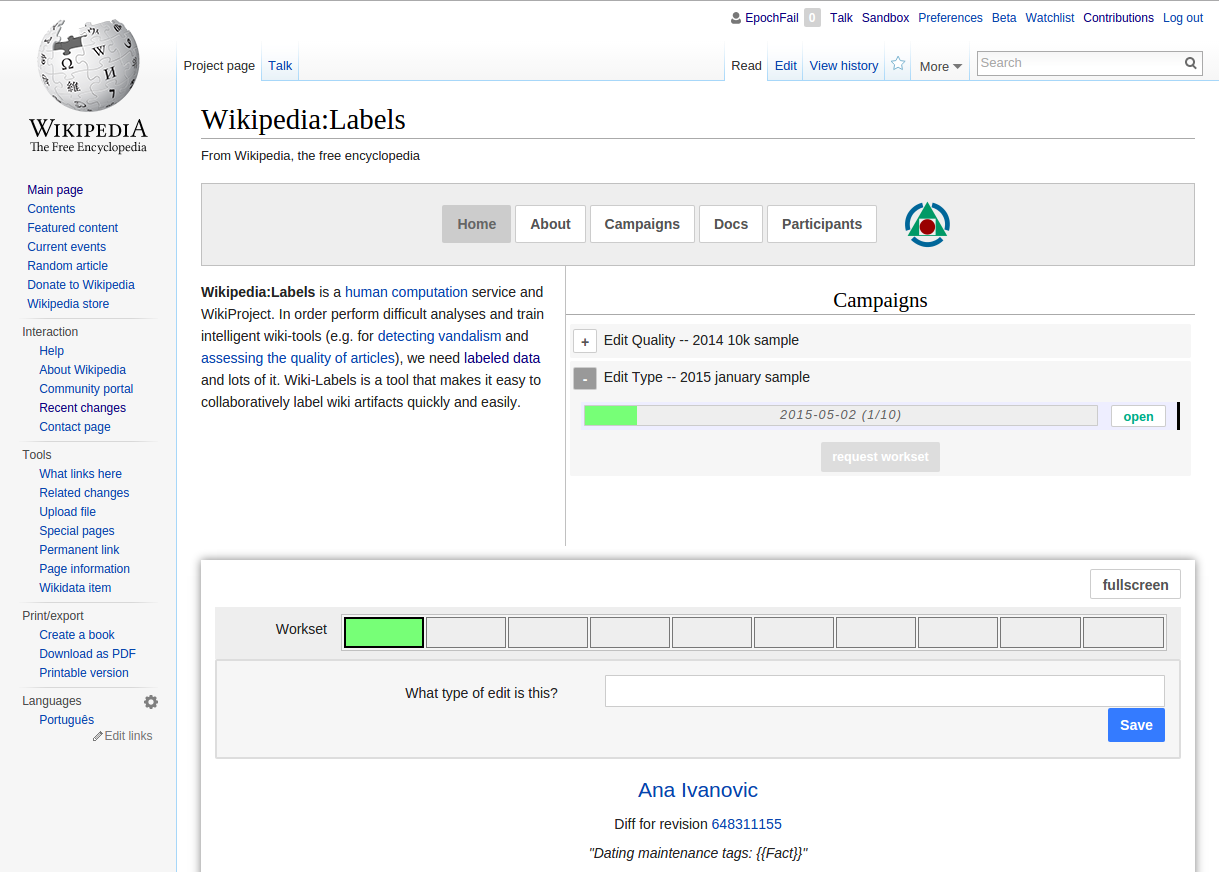
\includegraphics[width=.50\textwidth]{figures/Wiki_labels_gadget}
  \caption{The Wiki labels interface embedded in Wikipedia}
  \label{fig:wikilabels_screenshot}
\end{figure}

\leadin{Manual labeling campaigns with Wiki Labels}
We hold manual labeling by human Wikipedians as the gold standard for purposes of training a model to replicate human judgement.  By asking Wikipedians to demonstrate their judgement on examples from their own wikis, we can most closely tailor model predictions to match the judgements that make sense to these communities.  This contrasts with found data, which deceptively appears to be a better option because of its apparent completeness: every edit was either reverted or not.  In contrast, manual labeling has a high up-front expense of human labor.  To minimize that cost, we developed a high-speed, collaborative labeling interface called ``Wiki Labels\footnote{\url{http://enwp.org/:m:Wiki labels}}'' to allow Wikipedians to efficiently label large datasets.

For example, to supplement our models of edit quality, we replace the models based on ``reverted\_for\_damage'' found traces with judgments from a community labeling campaign, where we specifically ask labelers to distinguish ``damaging'' edits from ``good-faith'' edits. ``Good faith'' is a well-established term in Wikipedian culture\footnote{\url{https://enwp.org/WP:AGF}}, with specific local meanings that are different than their broader colloquial use---similar to how Wikipedians define ``consensus'' or ``neutrality''.  Using these labels we can build two separate models which allow users to filter for edits that are likely to be good-faith mistakes\cite{halfaker2017automated}, to just focus on vandalism, or to apply themselves broadly to all damaging edits.

\subsection{Dependency injection and interrogability}
One of the key features of ORES that allows scores to be generated in an efficient and flexible way is a dependency injection framework.  We use a dependency solver to determine what data is necessary for a scoring job and eventually compute the features used by a prediction model.

The flexibility provided by the dependency injection framework lets us implement a novel strategy for exploring \emph{how} ORES' models make predictions.  By exposing the features extracted to ORES users and allowing them to inject their own features, we can allow users to ask how predictions would change if the world were different.  Let's say you wanted to explore how ORES judges unregistered (anon) editors differently from registered editors.  Figure~\ref{fig:anon_injection} demonstrates two prediction requests to ORES.

\begin{figure*}[h]
\centering
\begin{subfigure}[t]{.5\textwidth}
  \makebox{\hrulefill}{
  \small
  \begin{verbatim}
  "damaging": {
    "score": {
      "prediction": false,
      "probability": {
        "false": 0.938910157824447,
        "true": 0.06108984217555305   }   }  }
  \end{verbatim}
  \hrule
  \normalsize}
  \caption{Prediction with \texttt{anon = false} injected}
  \label{fig:anon_injection_false}
\end{subfigure}~~
\begin{subfigure}[t]{.5\textwidth}
  \makebox{\hrulefill}{
  \small
  \begin{verbatim}
  "damaging": {
    "score": {
      "prediction": false,
      "probability": {
        "false": 0.9124151990561908,
        "true": 0.0875848009438092   }   }   }
  \end{verbatim}
  \hrule
  \normalsize}
  \caption{Prediction with \texttt{anon = true} injected}
  \label{fig:anon_injection_true}
\end{subfigure}
\caption{Two ``damaging'' predictions about the same edit are listed for ORES.  In one case, ORES is asked to make a prediction assuming the editor is unregistered (anon) and in the other, ORES is asked to assume the editor is registered.}
\label{fig:anon_injection}
\end{figure*}

Figure~\ref{fig:anon_injection_false} shows that ORES' ``damaging'' model concludes that the edit identified by the \emph{revision ID} of 34234210 is not damaging with 93.9\% confidence.  We can ask ORES to make a prediction about the exact same edit, but to assume that the editor was unregistered (anon). Figure~\ref{fig:anon_injection_true} shows the prediction if edit were saved by an anonymous editor.  ORES would still conclude that the edit was not damaging, but with less confidence (91.2\%).  By following a pattern like this for a single edit or a set of edits, we can get to know how ORES prediction models account for anonymity through experience with practical examples. Interrogability has also been used in creative new ways beyond bias explorations.  Some of our users have levered the feature injection system to expose \emph{hypothetical} predictions to support their work.  See the discussion of Ross's work recommendation tools in Section~\ref{sec:adoption_patterns}.


\section{Adoption patterns}
\label{sec:adoption_patterns}
When we designed and developed ORES, we were targeting a specific problem: expanding the set of values applied to the design of quality control tools to include a recent understanding of the importance of newcomer socialization.  We do not have any direct control of how developers chose to use ORES.  We hypothesize that, by making edit quality predictions available to all developers, we would lower the barrier to experimentation in this space.   After we deployed ORES, we implemented some basic tools to showcase ORES, but we observed a steady adoption of our various prediction models by external developers in current tools and through the development of new tools.\footnote{See complete list: \url{http://enwp.org/:mw:ORES/Applications}}

When we first released ORES, there was a wave of adoption in tools that were already used by Wikipedians.  Machine predictions proved useful as an addition to already-engineered systems used to support content patrolling work.  While this dynamic itself is fascinating, for the purposes of this paper, we focus on the development of new tools that use ORES that may not have been developed at all otherwise.  For example, the Wikimedia Foundation's product department developed a complete redesign on MediaWiki's Special:RecentChanges interface that implements a set of powerful filters and highlighting.  They took the ORES Review Tool to it's logical conclusion with an initiative that they referred to as Edit Review Improvements.\footnote{\url{http://enwp.org/:mw:Edit_Review_Improvements}}  In this interface, ORES scores are prominently featured at the top of the list of available filters, and they have been highlighted as one of the main benefits of the new interface to the editing community.

When we first developed ORES, English Wikipedia was the only wiki that we are aware of that had a fully-automated bot that used machine prediction to automatically revert obvious vandalism \cite{carter2008cluebot}.  After we deployed ORES, several wikis developed such bots of their own using ORES.  For example, PatruBOT in Spanish Wikipedia\footnote{\url{https://es.wikipedia.org/wiki/Usuario:PatruBOT}} and Dexbot in Persian Wikipedia\footnote{\url{https://fa.wikipedia.org/wiki/User:Dexbot}} now automatically revert edits that ORES predicts are damaging with high confidence. 

One of the most noteworthy new applications of ORES is the suite of tools developed by Sage Ross to support the Wiki Education Foundation's\footnote{\url{https://wikiedu.org/}} activities.  Their organization supports classroom activities that involve editing Wikipedia.  They develop tools and dashboards that help students contribute successfully and to help teachers monitor their students' work.  Ross has recently published about how he interprets meaning from ORES' article quality models \cite{ross2016visualizing} (an example of re-appropriation) and he has used the article quality model in their new editor support dashboard\footnote{\url{https://dashboard-testing.wikiedu.org}} in a novel way.  Specifically, Ross's tool\footnote{\url{https://dashboard-testing.wikiedu.org}} uses our feature injection system (see Section~\ref{sec:innovations_in_openness}) to suggest work to new editors.  This system asks ORES to score a student's draft article and then asking ORES to reconsider the predicted quality level of the article with \emph{one more header}, \emph{one more image}, or \emph{one more citation}. In doing so, Ross built an intelligent user interface that can expose the internal structure of a model in order to recommend the most productive development to the article---the change that will most likely bring it to a higher quality level.


\section{Case studies in reflection}
\label{sec:case_studies}
When we first deployed ORES, we reached out to several different wiki communities and invited them to test the system for use in patrolling for vandalism.  Before long, our users began filing false-positive reports on wiki pages of their own design --- some after our request, but mostly on their own.  In this section, we describe three cases where our users independently developed these false-positive reporting pages and how they used them to understand ORES, the roles of automated quality control in their own spaces, and to communicate with us about model bias.

\subsection{Patrolling/ORES (Italian Wikipedia)}
Italian Wikipedia was one of the first wikis where we deployed basic edit quality models.  Our local collaborator, who helped us develop the language specific features, User:Rotpunkt, created a page for ORES\footnote{\url{https://it.wikipedia.org/wiki/Progetto:Patrolling/ORES}} with a section for reporting false-positives (``falsi positivi'').  Within several hours, Rotpunkt and a few other editors noticed some trends.  These editors began to collect false positives under different headers representing themes they were seeing.  Through this process, editors from Italian Wikipedia were effectively performing an inductive, grounded theory-esque exploration of ORES errors, trying to identify themes and patterns in the errors that ORES was making.

One of the themes they identified fell under the header: ``corrections to the verb for \emph{have}'' (``correzioni verbo avere'').  It turns out that the word ``ha'' in Italian translates to the English verb ``to have''.  In English and many other languages, ``ha'' signifies laughing, and it generally is not a phrase found in encyclopedic prose. In addition, most language versions of Wikipedia tend to have at least some amount of English-language vandalism.  We had built a common feature in the damage model called ``informal words'' that captured these types of patterns.  But in this case, it was clear that in Italian ``ha'' should not carry signal of vandalism, while ``hahaha'' still should. Because of the work of Rotpunkt and his collaborators in Italian Wikipedia, we were able to recognize the source of this issue (a set of features intended to detect the use of \emph{informal language} in articles) and to remove ``ha'' from that list for Italian Wikipedia.

\subsection{PatruBOT (Spanish Wikipedia)}
Soon after we released support for Spanish Wikipedia, a volunteer developer made a bot to automatically revert edits using ORES's predictions for the ``damaging'' model (PatruBOT).  This bot was not running for long before our discussion spaces were bombarded with confused Spanish-speaking editors asking us why ORES did not like their work.  We struggled to understand the complaints until someone told us about PatruBOT. 

We found that this case was one of tradeoffs between precision/recall and false positives/negatives---a common issue with machine learning applications. We concluded that PatruBOT's threshold for reverting was too sensitive. ORES reports a classification and a probability score, but it is up to the developers to decide if, for example, the bot will only auto-revert edits classified as damage with a .90, .95, .99, or higher likelihood estimate. A higher threshold will minimize the chance a good edit will be mistakenly auto-reverted, but also increase the chance that a bad edit will not be auto-reverted.  Ultimately, our view was that each volunteer community should decide where to draw the line between false positives and false negatives, but we could help inform their discussion.

The Spanish Wikipedians who were concerned with these issues began a discussion about PatruBOT's activities and blocked the bot until the issue was sorted. Using wiki pages, they organized an crowdsourced evaluation of the fitness of PatruBOT's behavior\footnote{\url{https://es.wikipedia.org/wiki/Wikipedia:Mantenimiento/Revisi\%C3\%B3n_de_errores_de_PatruBOT\%2FAn\%C3\%A1lisis}}.  This evaluation and discussion is ongoing, \footnote{\url{https://es.wikipedia.org/wiki/Wikipedia:Caf\%C3\%A9\%2FArchivo\%2FMiscel\%C3\%A1nea\%2FActual\#Parada_de_PatruBOT}} but it shows how stakeholders do not need to have an advanced understanding in machine learning evaluation to meaningfully participate in a sophisticated discussion about how, when, why, and under what conditions such classifiers should be used. Because of the API-based design of the ORES system, no actions are needed on our end once they make a decision, as the fully-automated bot is developed and governed by Spanish Wikipedians.

\subsection{Bias against anonymous editors}
\begin{figure*}[h!]
\centering
\begin{subfigure}[t]{.33\textwidth}
  \centering
  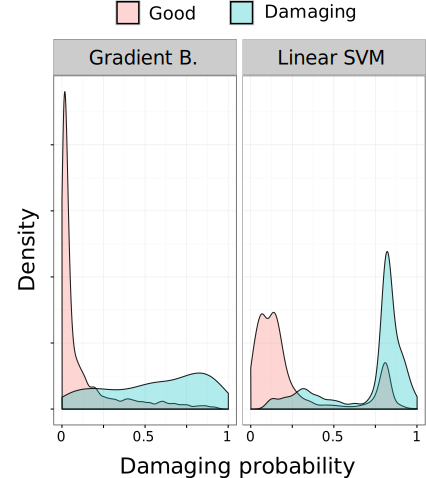
\includegraphics[width=.85\textwidth]{figures/natural_damaging_gb_vs_svc}
  \caption{No injected features}
  \label{fig:natural_damaging_gb_bs_svc}
\end{subfigure}~~
\begin{subfigure}[t]{.33\textwidth}
  \centering
  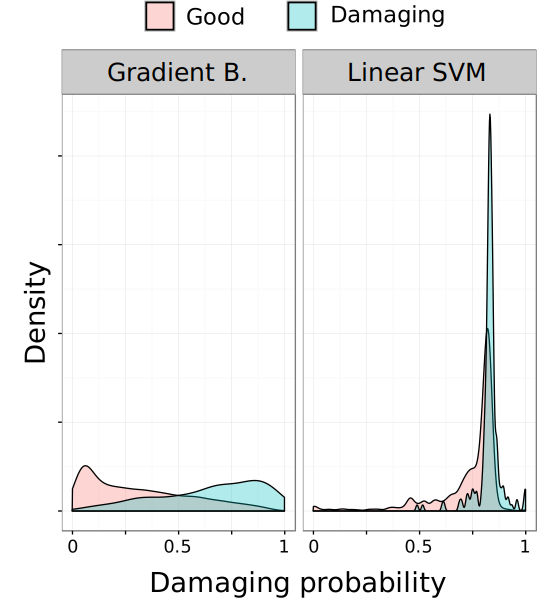
\includegraphics[width=.85\textwidth]{figures/anon_damaging_gb_vs_svc}
  \caption{Everyone is anonymous}
  \label{fig:anon_damaging_gb_bs_svc}
\end{subfigure}~~
\begin{subfigure}[t]{.33\textwidth}
  \centering
  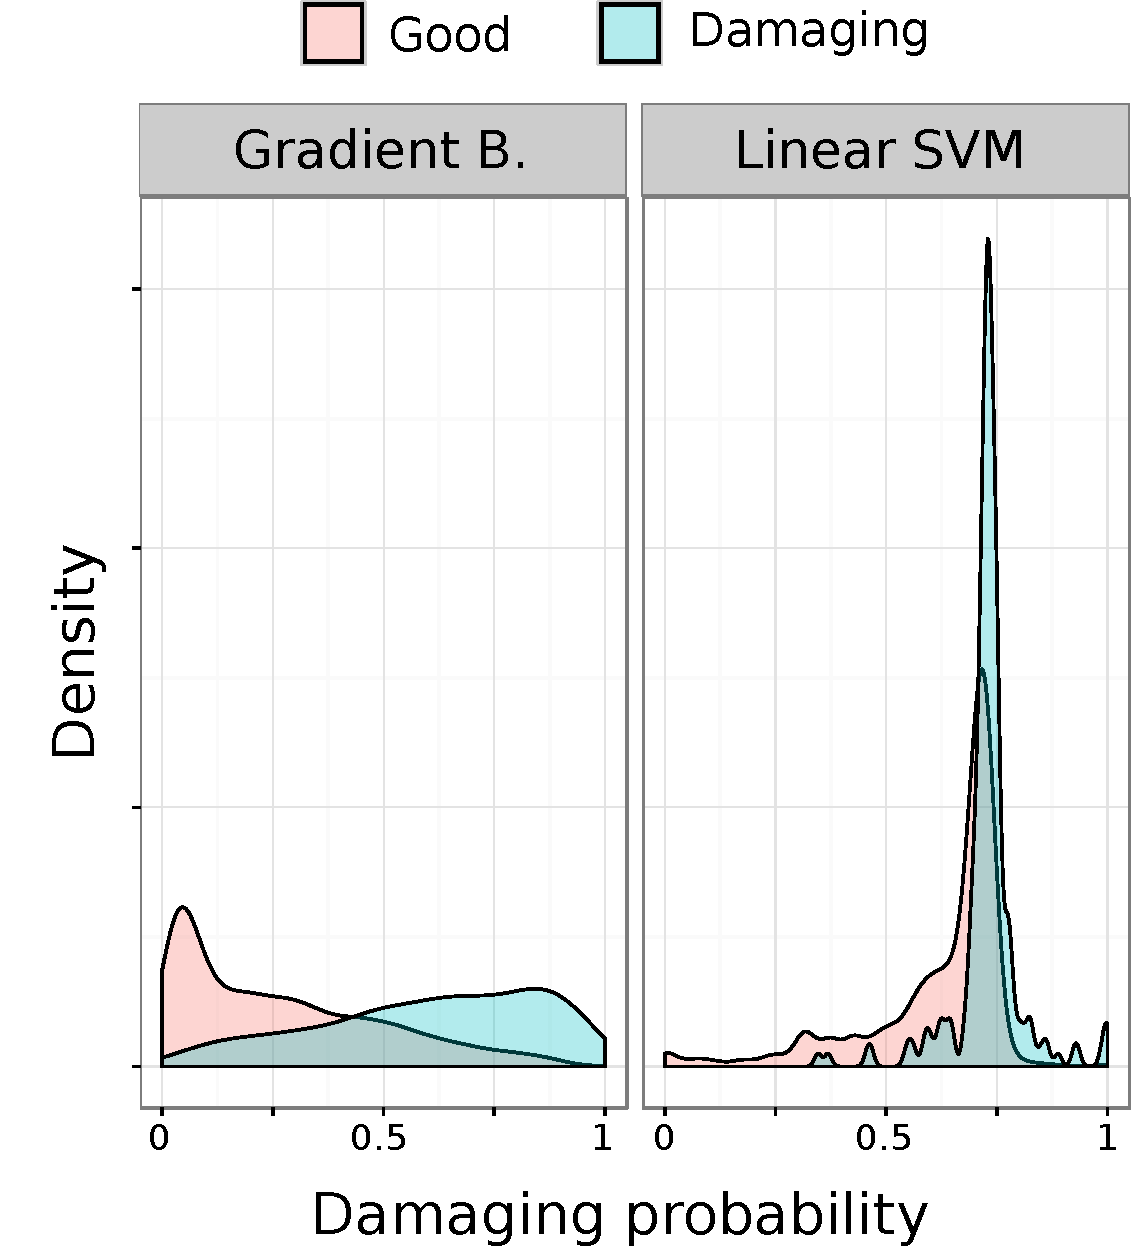
\includegraphics[width=.85\textwidth]{figures/newcomer_damaging_gb_vs_svc}
  \caption{Everyone is newly registered}
  \label{fig:newcomer_damaging_gb_bs_svc}
\end{subfigure}
\caption{The distributions of the probability of a single edit being scored as ``damaging'' based on injected features for the target user-class is presented.  Note that when injecting user-class features (anon, newcomer), all other features are held constant.}
\label{fig:prediction_error_for_anons_and_newcomers}
\end{figure*}

Shortly after we deployed ORES, we received reports that ORES's damage detection models were overly biased against anonymous editors.  At the time, we were using Linear SVM\footnote{\url{http://scikit-learn.org/stable/modules/generated/sklearn.svm.LinearSVC.html}} estimators to build classifiers, and we were considering making the transition towards ensemble strategies like GradientBoosting and RandomForest estimators.\footnote{\url{http://scikit-learn.org/stable/modules/ensemble.html}}  We took the opportunity to look for bias in the error of estimation between anonymous editors and newly registered editors.  By using our feature injection/interrogation strategy (described in Section~\ref{sec:innovations_in_openness}), we could ask our current prediction models how they would change their predictions if the exact same edit were made by a different editor.

Figure~\ref{fig:prediction_error_for_anons_and_newcomers} shows the probability density of the likelihood of ``damaging'' given three different passes over the exact same test set, using two of our modeling strategies.  Figure~\ref{fig:natural_damaging_gb_bs_svc} shows that, when we leave the features to their natural values, it appears that both models are able to differentiate effectively between damaging edits (high-damaging probability) and non-damaging edits (low-damaging probability) with the odd exception of a large amount of non-damaging edits with a relatively high-damaging probability around 0.8 in the case of the Linear SVM model.  Figures~\ref{fig:anon_damaging_gb_bs_svc} and \ref{fig:newcomer_damaging_gb_bs_svc} show a stark difference.  For the scores that go into these plots, characteristics of anonymous editors and newly registered editors were injected for all of the test edits.  We can see that the GradientBoosting model can still differentiate damage from non-damage while the Linear SVM model flags nearly all edits as damage in both case.

Through the reporting of this issue and our subsequent analysis, we were able to identify the weakness of our estimator and show that an improvement to our modeling strategy mitigates the problem.  Without such a tight feedback loop, we most likely would not have noticed how poorly ORES's damage detection models were performing in practice.  Worse, it might have caused vandal fighters to be increasingly (and inappropriately) skeptical of contributions by anonymous editors and newly registered editors---two groups of contributors that are already met with unnecessary hostility\footnote{\url{http://enwp.org/:en:Wikipedia:IPs_are_human_too}}\cite{halfaker2013rise}.


\section{Conclusion and future work}
\label{sec:conclusions_and_future_work}
ORES as a socio-technical system has helped us 1) refine our understandings of volunteers' needs across wiki communities, 2) identify and address biases in ORES's models, and 3) reflect on how people think about what types of automation they find acceptable in their \emph{spaces}.  Through our participatory design process with various Wikipedian communities, we have arrived at several innovations in open machine learning practice that represent advancements in the field.

As we stated in Section~\ref{sec:design_rationale}, we measure success in new conversations about how algorithmic tools affect editing dynamics, as well as new types of tools that take advantage of these resources, implementing alternative visions of what Wikipedia is and ought to be.  We have demonstrated through discussion of adoption patterns and case studies in reflection around the use of algorithmic systems that something fundamental is \emph{working}.  ORES is being heavily adopted.  The meaning of ORES models is being re-appropriated.  Both the models and the technologies that use the models are being collaboratively audited by their users and those who are affected.

\subsection{Participatory machine learning}
In a world increasingly dominated by for-profit content platforms --- often marketed by their corporate owners as ``communities'' \cite{gillespie2018custodians} --- Wikipedia is an anomaly. While the non-profit Wikimedia Foundation has only a fraction of the resources as Facebook or Google, the unique principles and practices in the broad Wikipedia/Wikimedia movement are a generative constraint. ORES emerged out of this context, operating at the intersection of a pressing need to deploy efficient machine learning at scale for content moderation, but to do so in ways that enable volunteers to develop and deploy advanced technologies on their own terms. Our approach is in stark contrast to the norm in machine learning research and practice, which involves a more top-down mode of developing the most precise classifiers for a known ground truth, then wrap those classifiers in a complete technology for end-users, who must treat them as black boxes.

The more wiki-inspired approach to what we call ``participatory machine learning'' imagines classifiers to be just as provisional and open to skeptical reinterpretation as the content of Wikipedia's encyclopedia articles. And like Wikipedia articles, we suspect some classifiers will be far better than others based on how volunteers develop and curate them, for various definitions of ``better'' that are already being actively debated. Our case studies briefly indicate how volunteers have collectively engaged in sophisticated discussions about how they ought to use machine learning. ORES' fully open, reproducible, and audit-able code and data pipeline---from training data to models to scored predictions---enables a wide range of new collaborative practices. ORES is a more socio-technical approach to issues in FATML, where attention is often placed on technical solutions, like interactive visualizations for model interpretability or mathematical guarantees of operationalized definitions of fairness. Our approach is specific to the particular practices and values of Wikipedia, and we have shown how ORES has been developed to fit into this context.

ORES also represents an innovation in openness in that it decouples several activities that have typically all been performed by engineers or under their direct supervision: choosing or curating training data, building models to serve predictions, auditing predictions for false positives/negatives, and developing interfaces or automated agents that act on those predictions. Often, those who develop and maintain the technical infrastructure for systems gain what we can call an \textit{incidental jurisdiction} over the other areas, which does not necessarily require that same expertise. As our cases have shown, people with extensive contextual and domain expertise in an area can make well-informed decisions about curating training data, identifying false positives/negatives, setting thresholds, and designing interfaces that use scores from a classifier. In decoupling these actions, ORES helps delegate these responsibilities more broadly, opening up the structure of the socio-technical system and expanding who can participate in it.

\subsection{Critical reflection}
In section~\ref{sec:case_studies}, we showed evidence of critical reflection on the current processes and the role of algorithms in quality control.  These case studies show that collaborative auditing is taking place, that there is a proliferation of tools based on alternative uses of ORES we did not imagine, and that that Wikipedians have more agency over their quality control processes. We also see an important expansion into supporting non-English language Wikipedias, which have historically not received as much support in this area. We are inspired by much of the concern that has surfaced for looking into biases in ORES' prediction models (e.g. anon bias and the Italian ``ha'') and over what role algorithms should have in directly reverting human actions (e.g. PatruBOT and Dexbot).

Eliciting this type of critical reflection and empowering users to engage in their own choices about the roles of algorithmic systems in their social spaces has typically been more of a focus from the Critical Algorithms Studies literature, which comes from a more humanistic and interpretivist social science perspective (e.g. \cite{barocas2013governing, kitchin2017thinking}. This literature also emphasizes a need to see algorithmic systems as dynamic and constantly under revision by developers \cite{seaver2017algorithms} --- work that is invisible in most platforms, but is foregrounded in ORES. In these case studies, we see that given ORES' open API and Wikipedia's collaborative wiki pages, Wikipedians will audit ORES' predictions and collaborate with each other to build information about trends in ORES' mistakes and how they expected their own processes to function.

\subsection{Future work}
Observing ORES in practice suggests avenues of future work toward crowd-based auditing tools.  As our case studies suggest, auditing of ORES' predictions and mistakes has become a popular activity.  Even though we did not design interfaces for discussion and auditing, some Wikipedians have used unintended affordances of wiki pages and MediaWiki's template system to organize processes for flagging false positives and calling them to our attention.  This process has proved invaluable for improving model fitness and addressing critical issues of bias against disempowered contributors.  To better facilitate this process, future system builders should implement structured means to refute, support, discuss, and critique the predictions of machine models.  With a structured way to report what machine prediction gets right and wrong, we can make it easier for tools that use ORES to also allow for reporting mistakes and for others to infer trends.  For example, a database of ORES mistakes could be queried in order to build the kind of thematic analyses that Italian Wikipedians showed us (see section~\ref{sec:case_studies}).  By supporting such an activity, we are working to transfer more power from ourselves and to our users.  Should one of our models develop a nasty bias, our users will be more empowered to coordinate with each other, show that the bias exists and where it causes problems, and either get the model's predictions turned off or even shut down the use of ORES (e.g. PatruBOT).

We also look forward to what those from the FATML and CAS fields can do with ORES, which is far more open than most high-scale machine learning applications. Most of the studies and critiques of \emph{subjective algorithms}\cite{tufekci2015algorithms} focus on for-profit organizations that are strongly resistant to external interrogation. Wikipedia is one of the largest and arguably most impactful information resources in the world, and decisions about what is and is not represented have impacts across all sectors of society.  The algorithms that ORES makes available are part of the decision process that leads to some people's contributions remaining and others being removed.  This is a context where \emph{algorithms matter to humanity}, and we are openly experimenting with the kind of transparent and open processes that \emph{fairness and transparency in machine learning} researchers are advocating.  Yet, we have new problems and new opportunities.  There is a large body of work exploring how biases manifest and how unfairness can play out in algorithmically mediated social contexts.  ORES would be an excellent place to expand the literature within a specific and important field site.

Finally, we also see potential in allowing Wikipedians to freely train, test, and use their own prediction models without our engineering team involved in the process.  Currently, ORES is only suited to deploy models that are trained and tested by someone with a strong modeling and programming background, and we currently do that work for those who come to us with a training dataset and ideas about what kind of classifier they want to build.  That does not necessarily need to be the case.  We have been experimenting with demonstrating ORES model building processes using Jupyter Notebooks\footnote{\url{http://jupyter.org}} \footnote{e.g. \url{ https://github.com/wiki-ai/editquality/blob/master/ipython/reverted_detection_demo.ipynb}} and have found that new programmers can understand the work involved.  This is still not the holy grail of crowd-developed machine prediction, where all of the incidental complexities involved in programming are removed from the process of model development and evaluation.  Future work exploring strategies for allowing end-users to build models that are deployed by ORES would surface the relevant HCI issues involved and the changes to the technological conversations that such a margin-opening intervention might provide.


\section{Acknowledgements}
\label{sec:acknowledgements}
REDACTED FOR REVIEW


\section{Appendix}
See the supplementary material for the Appendix section.

% Bibliography
\bibliographystyle{ACM-Reference-Format}
\bibliography{refs}

\pagebreak
\appendix
\section{Appendix}
\label{sec:appendix}
\subsection{ORES system engineering}
\label{sec:ores_system_engineering}
In this section we describe how the system was designed in order to meet the needs of Wikipedian work practices and the tools that support them.

\subsubsection{Scaling \& robustness}
To be useful for Wikipedians and tool developers, ORES uses distributed computation strategies to provide a robust, fast, high-availability service.  Reliability is a critical concern in Wikipedian quality control work.  Interruptions in Wikipedia's algorithmic systems have historically led to increased burdens for human workers and a higher likelihood that readers will see vandalism\cite{geiger2013levee}.  Further, ORES needs to scale to be able to be used in multiple different tools across different language Wikipedias where its predecessors only needed to scale for use in a single tool.

This horizontal scaleability is achieved in two ways: input-output (IO) workers (uwsgi\footnote{\url{https://uwsgi-docs.readthedocs.io/}}) and the computation (CPU) workers (celery\footnote{\url{http://www.celeryproject.org/}}).  Requests are split across available IO workers, and all necessary data is gathered using external APIs (e.g. the MediaWiki API\footnote{\url{http://enwp.org/:mw:MW:API}}).  The data is then split into a job queue managed by \emph{celery} for the CPU-intensive work.  This efficiently uses available resources and can dynamically scale, adding and removing new IO and CPU workers in multiple datacenters as needed.  This is also fault-tolerant, as servers can fail without taking down the service as a whole.

\subsubsection{Real-time processing}
The most common use case of ORES is real-time processing of edits to Wikipedia immediately after they are saved.  For example, those using counter-vandalism tools like Huggle monitor edits within seconds of when they are made.  It is critical that ORES return these requests in a timely manner.  We implement several strategies to optimize this request pattern.

\leadin{Single score speed}
In the worst case scenario, ORES is generating a score from scratch.  This is the common case when a score is requested in real-time---which invariably occurs right after the target edit or article is saved.  We work to ensure that the median score duration is around 1 second so that counter-vandalism efforts are not substantially delayed(c.f. \cite{geiger2013levee}).  Our metrics tracking currently suggests that for the week April 6-13th, 2018, our median, 75\%, and 95\% score response timings are 1.1, 1.2, and 1.9 seconds respectively.

\leadin{Caching and precaching}
In order to take advantage of our users' overlapping interests in scoring recent activity, we also maintain a basic least-recently-used (LRU) cache\footnote{Implemented natively by Redis, \url{https://redis.io}} using a deterministic score naming scheme (e.g. \texttt{enwiki:123456:damaging} would represent a score needed for the English Wikipedia damaging model for the edit identified by 123456).  This allows requests for scores that have recently been generated to be returned within about 50ms via HTTPS.  In other words, a request for a recent edit that had previously been scored is 20X faster due to this cache.

In order to make sure that scores for \emph{all recent edits} are available in the cache for real-time use cases, we implement a ``precaching'' strategy that listens to a high-speed stream of recent activity in Wikipedia and automatically requests scores for a specific subset of actions (e.g. edits).  With our LRU and precaching strategy, we consistently attain a cache hit rate of about 80\%.

\leadin{De-duplication}
In real-time ORES use cases, it's common to receive many requests to score the same edit/article right after it was saved.  We use the same deterministic score naming scheme from the cache to identify scoring tasks, and ensure that simultaneous requests for that same score are de-duplicated.  This allows our service to trivially scale to support many different robots and tools on the same wiki.

\subsubsection{Batch processing}
Many different types of Wikipedia's bots rely on periodic, batch processing strategies to support Wikipedian work processes\cite{geiger2011lives}.  For example, many bots are designed to build worklists for Wikipedia editors (e.g. \cite{cosley2007suggestbot}) on a daily or weekly basis, and many of these tools have adopted ORES to include an article quality prediction for use in prioritization of work (see section~\ref{sec:adoption_patterns}).  Work lists are either built from the sum total of all 5m+ articles in Wikipedia, or from some large subset specific to a single WikiProject (e.g. WikiProject Women Scientists claims about 6k articles\footnote{As demonstrated by \url{https://quarry.wmflabs.org/query/14033}}).  We've observed robots submitting large batch processing jobs to ORES once per day.  It's relevant to note that many researchers are also making use of ORES for various analyses, and their activity usually shows up in our logs as a similar burst of requests.

In order to most efficiently support this type of querying activity, we implemented batch optimizations in ORES by splitting IO and CPU operations into distinct stages.  During the IO stage, all data is gathered for all relevant scoring jobs in batch queries.  During the CPU stage, scoring jobs are split across our distributed processing system.  This batch processing affords up to a 5X increase in time to scoring speed for large requests\cite{sarabadani2017building}.  At this rate, a user can request 10s of million of scores in less than 24 hours in the worst case scenario (no scores were cached) without substantially affecting the service for others.

\subsubsection{Empirical access patterns}
\label{sec:appendix.empirical_access_patterns}
\begin{figure}[h]
\centering
\begin{subfigure}[t]{\columnwidth}
  \centering
  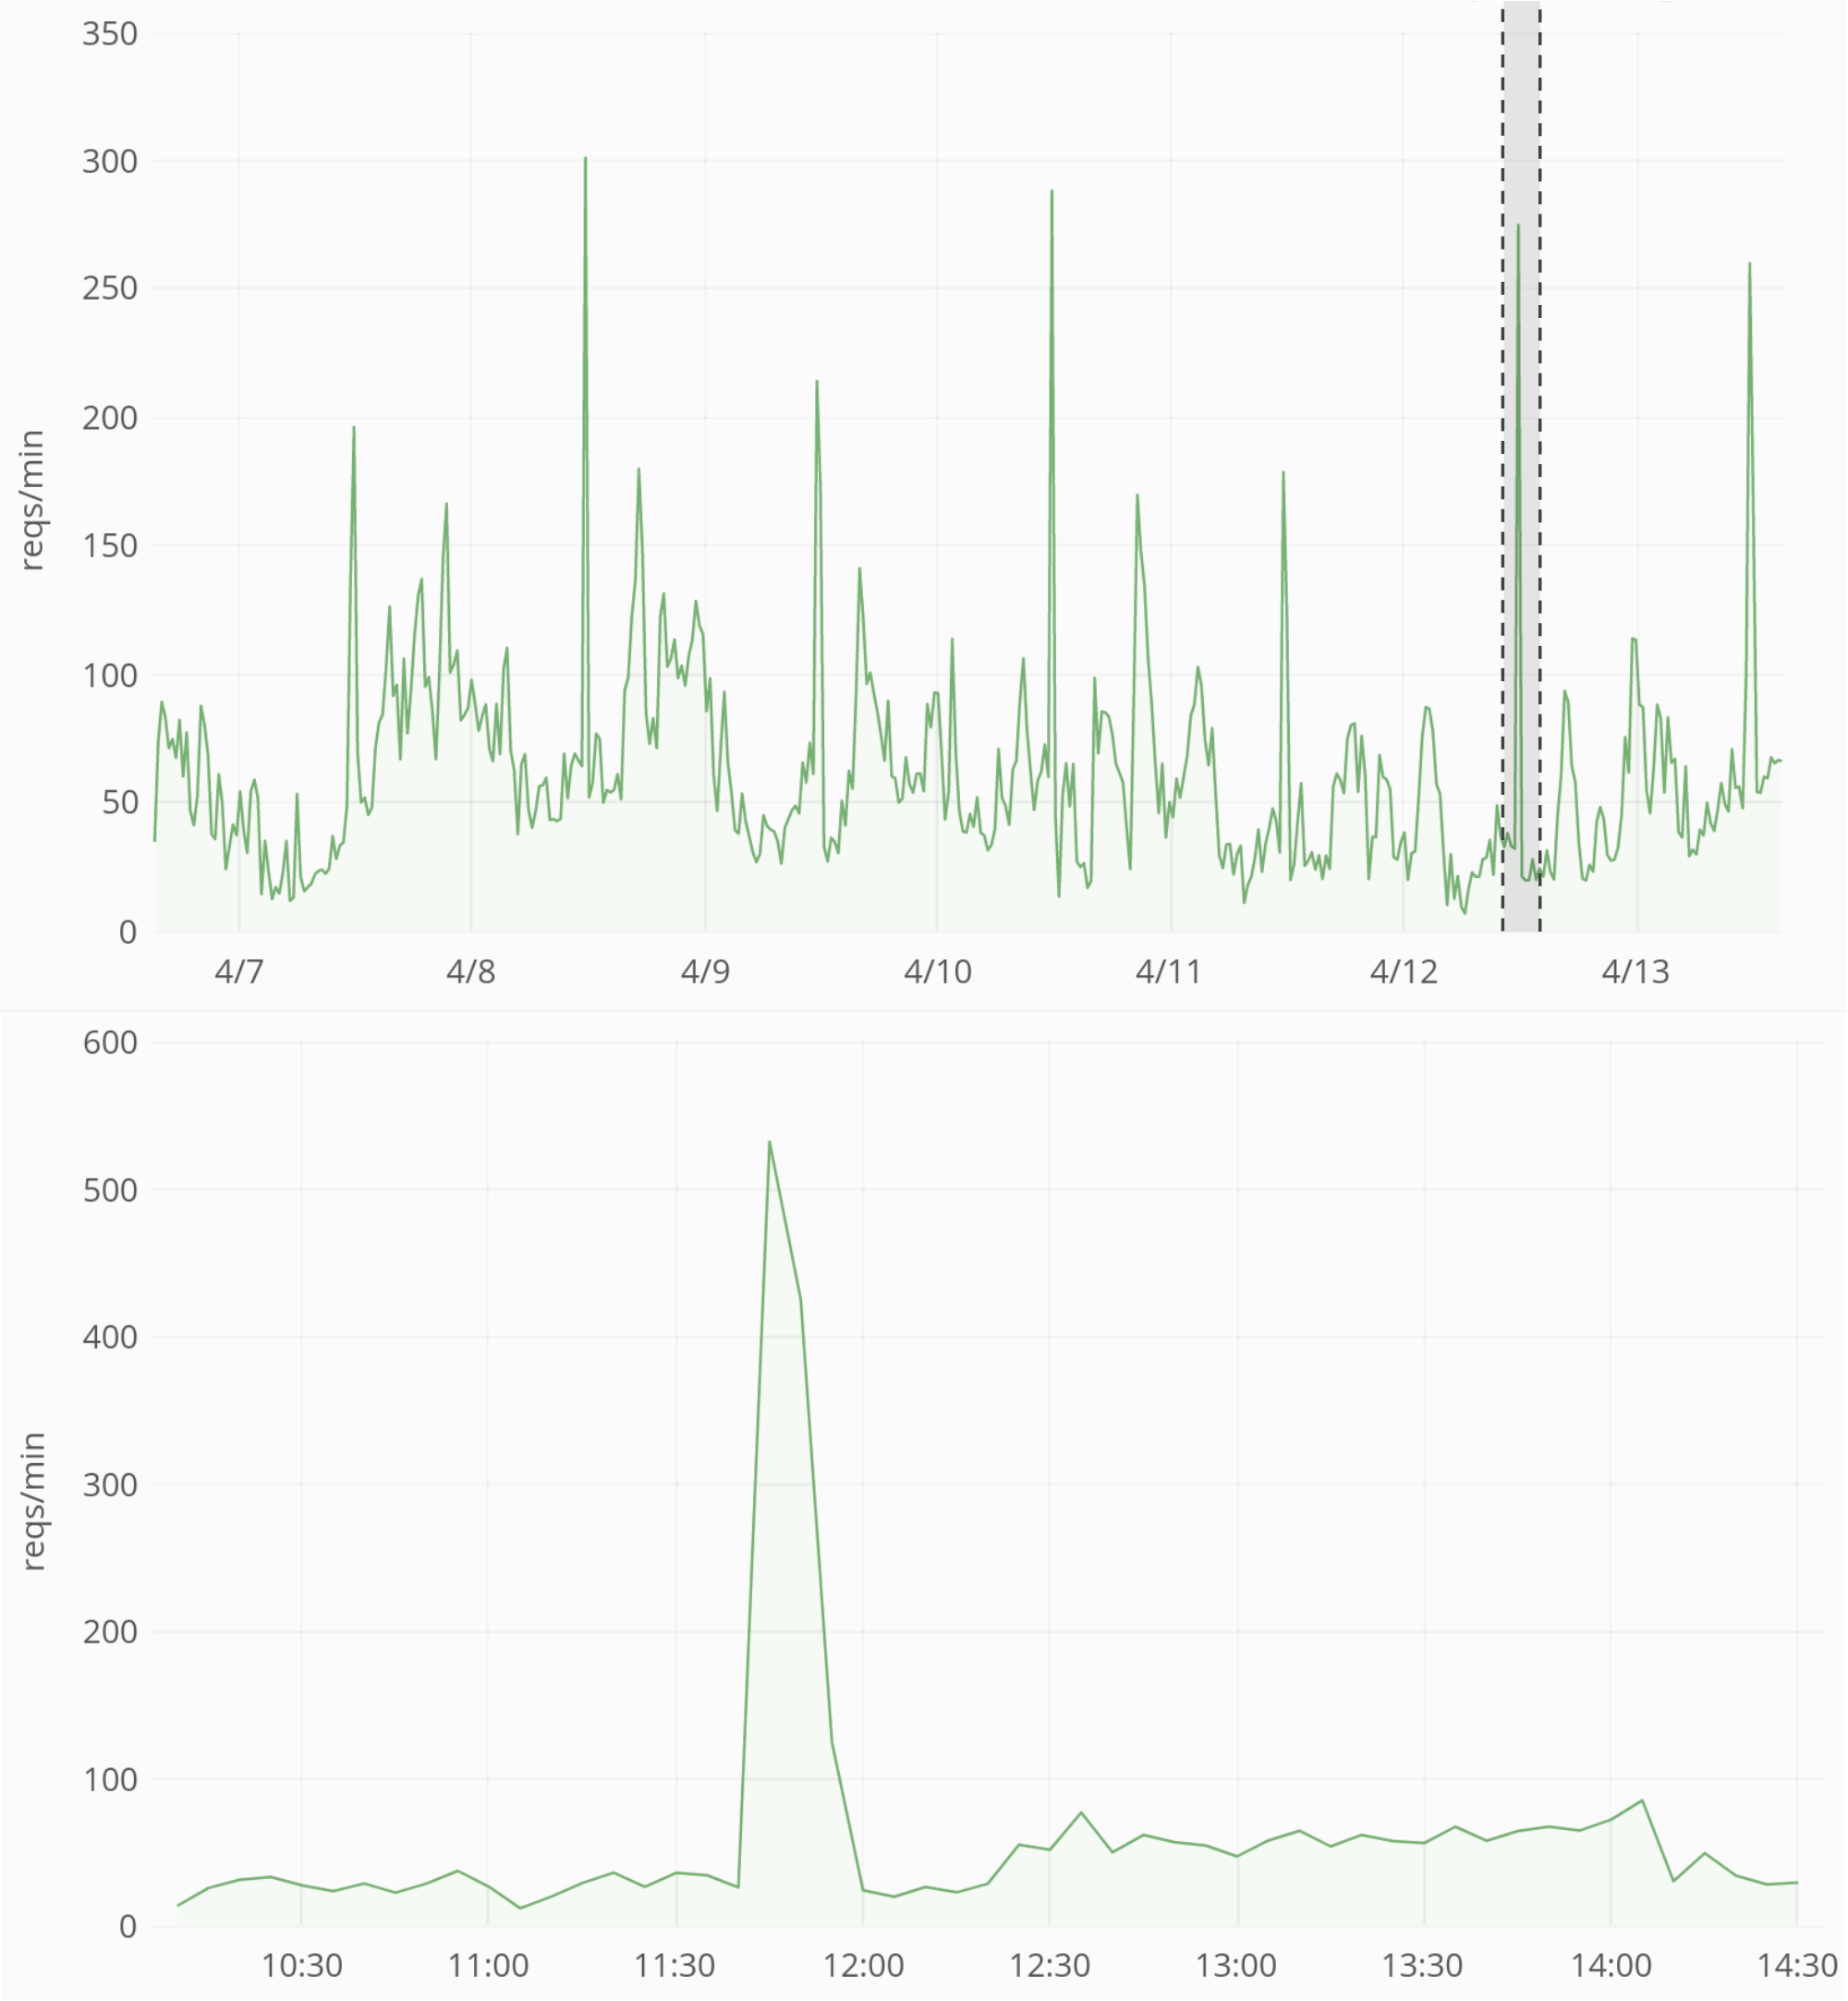
\includegraphics[width=.95\textwidth]{figures/ORES_request_activity_201804_week_vs_4hours}
  \caption{External requests per minute with a 4 hour block broken out to highlight a sudden burst of requests}
  \label{fig:ores_request_rate}
\end{subfigure}\\
\begin{subfigure}[t]{\columnwidth}
  \centering
  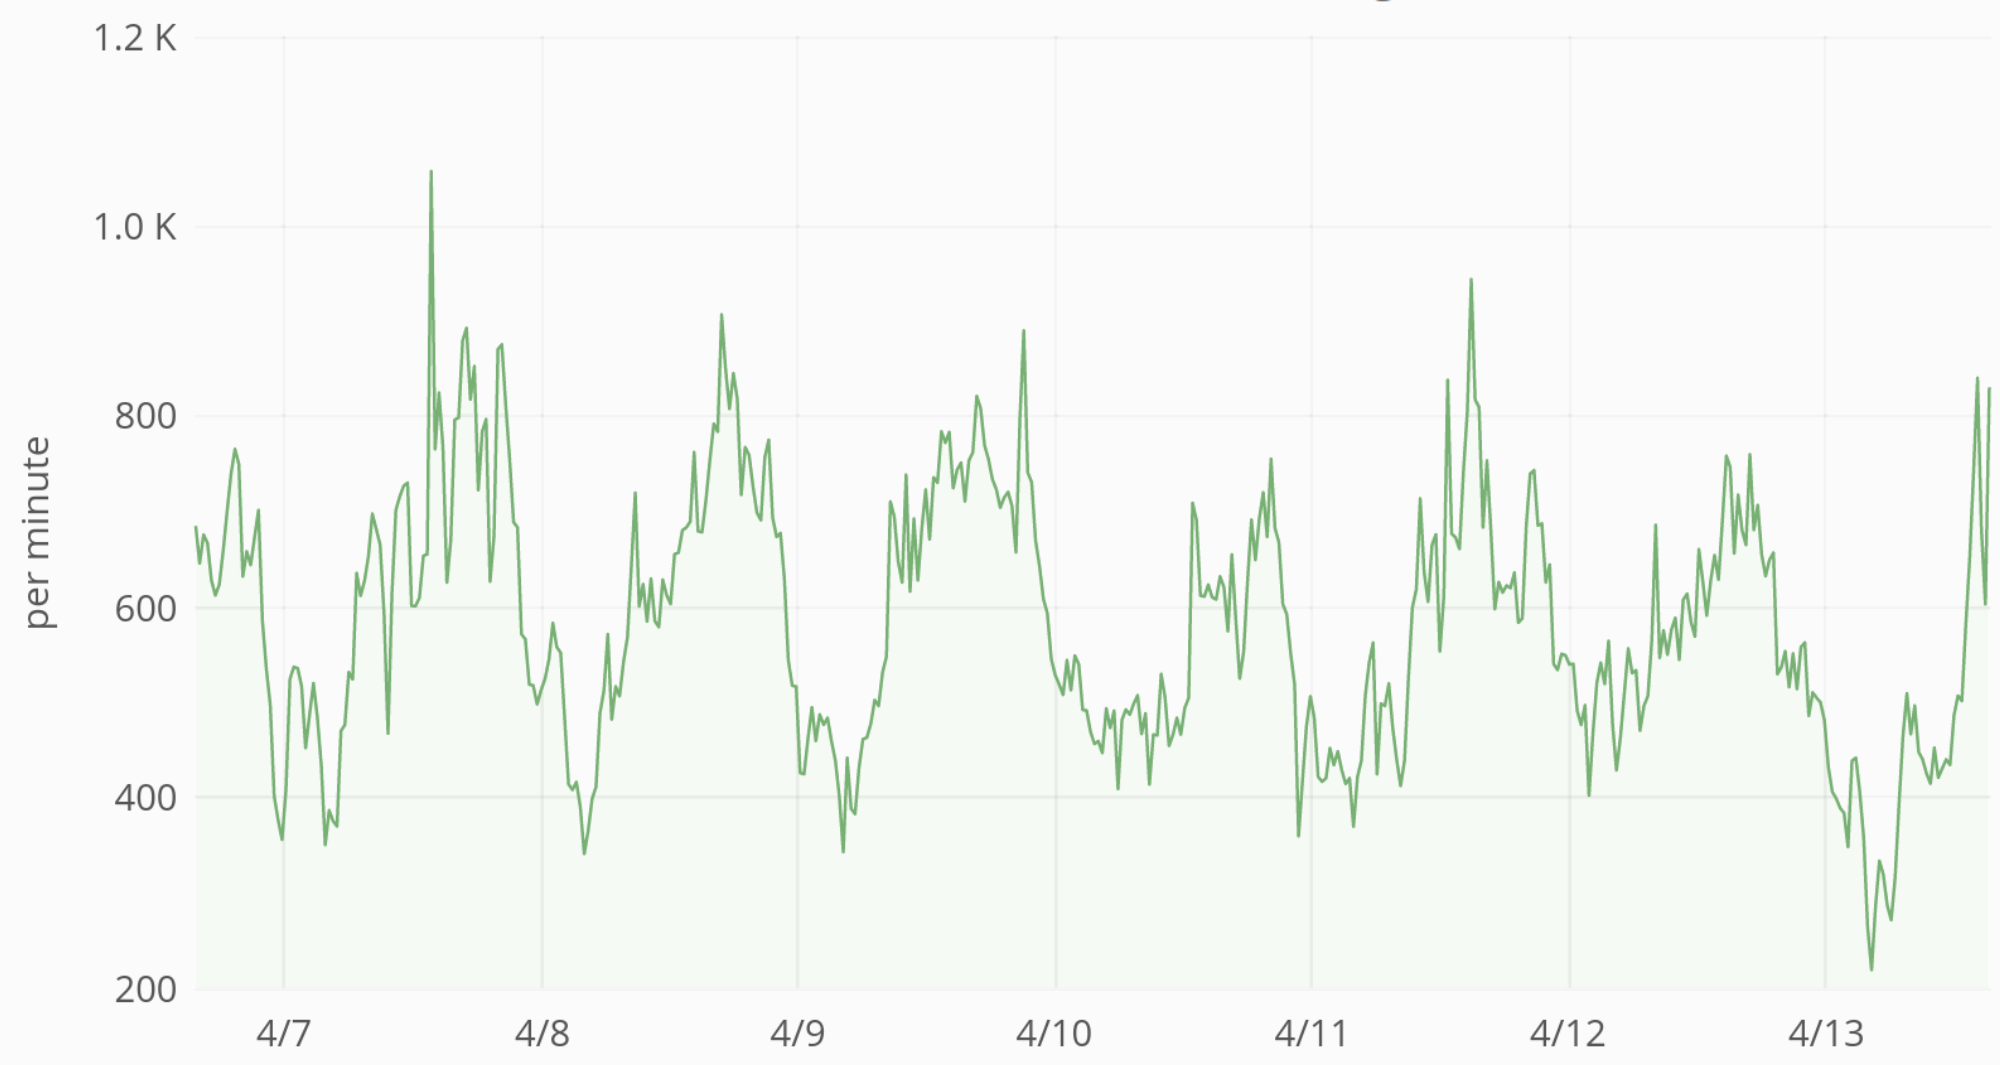
\includegraphics[width=.95\textwidth]{figures/ORES_precache_request_rate_201804}
  \caption{Precaching requests per minute}
  \label{fig:ores_precache_rate}
\end{subfigure}
\caption{Request rates to the ORES service for the week ending on April 13th, 2018}
\label{fig:ores_activity}
\end{figure}


The ORES service has been online since July 2015\cite{halfaker2015artificial}.  Since then, usage has steadily risen as we've developed and deployed new models and additional integrations are made by tool developers and researchers.  Currently, ORES supports 78 different models and 37 different language-specific wikis.

Generally, we see 50 to 125 requests per minute from external tools that are using ORES' predictions (excluding the MediaWiki extension that is more difficult to track).  Sometimes these external requests will burst up to 400-500 requests per second.  Figure~\ref{fig:ores_request_rate} shows the periodic and ``bursty'' nature of scoring requests received by the ORES service.  For example, every day at about 11:40 UTC, the request rate jumps---most likely a batch scoring job such as a bot.

Figure~\ref{fig:ores_precache_rate} shows the rate of precaching requests coming from our own systems.  This graph roughly reflects the rate of edits that are happening to all of the wikis that we support since we'll start a scoring job for nearly every edit as it happens.  Note that the number of precaching requests is about an order of magnitude higher than our known external score request rate.  This is expected, since Wikipedia editors and the tools they use will not request a score for every single revision.  This is a computational price we pay to attain a high cache hit rate and to ensure that our users get the quickest possible response for the scores that they \emph{do} need.

Taken together these strategies allow us to optimize the real-time quality control workflows and batch processing jobs of Wikipedians and their tools.  Without serious effort to make sure that ORES is practically fast and highly available to real-time use cases, ORES would become irrelevant to the target audience and thus irrelevant as a boundary-lowering intervention.  By engineering a system that conforms to the work-process needs of Wikipedians and their tools, we've built a systems intervention that has the potential gain wide adoption in Wikipedia's technical ecology.

\subsection{Explicit pipelines}
\label{sec:appendix.explicit_pipelines}
We have designed the process of training and deploying ORES prediction models to be repeatable and reviewable.  Consider the code shown in figure~\ref{fig:english_damaging_makefile} that represents a common pattern from our model-building Makefiles.

Essentially, this code helps someone determine where the labeled data comes from (manually labeled via the Wiki Labels system).  It makes it clear how features are extracted (using the \texttt{revscoring extract} utility and the \texttt{feature\_lists.enwiki.damaging} feature set).  Finally, this dataset of extracted features is used to cross-validate and train a model predicting the ``damaging'' label and a serialized version of that model is written to a file.  A user could clone this repository, install the set of requirements, and run \texttt{make enwiki\_models} and expect that all of the data-pipeline would be reproduced, and an equivalent model obtained.

By explicitly using public resources and releasing our utilities and Makefile source code under an open license (MIT), we have essentially implemented a turn-key process for replicating our model building and evaluation pipeline.  A developer can review this pipeline for issues knowing that they are not missing a step of the process because all steps are captured in the Makefile.  They can also build on the process (e.g. add new features) incrementally and restart the pipeline.  In our own experience, this explicit pipeline is extremely useful for identifying the origin of our own model building bugs and for making incremental improvements to ORES' models.

At the very base of our Makefile, a user can run \texttt{make models} to rebuild all of the models of a certain type.  We regularly perform this process ourselves to ensure that the Makefile is an accurate representation of the data flow pipeline.  Performing complete rebuild is essential when a breaking change is made to one of our libraries.  The resulting serialized models are saved to the source code repository so that a developer can review the history of any specific model and even experiment with generating scores using old model versions.

\begin{figure}[h]
        \makebox{\hrulefill}{
        \small
        \begin{verbatim}
datasets/enwiki.human_labeled_revisions.20k_2015.json:
    ./utility fetch_labels \
        https://labels.wmflabs.org/campaigns/enwiki/4/ > $@

datasets/enwiki.labeled_revisions.w_cache.20k_2015.json: \
        datasets/enwiki.labeled_revisions.20k_2015.json
    cat $< | \
        revscoring extract \
            editquality.feature_lists.enwiki.damaging \
            --host https://en.wikipedia.org \
            --extractor $(max_extractors) \
            --verbose > $@

models/enwiki.damaging.gradient_boosting.model: \
        datasets/enwiki.labeled_revisions.w_cache.20k_2015.json
    cat $^ | \
    revscoring cv_train \
        revscoring.scoring.models.GradientBoosting \
        editquality.feature_lists.enwiki.damaging \
        damaging \
        --version=$(damaging_major_minor).0 \
        -p 'learning_rate=0.01' \
        -p 'max_depth=7' \
        -p 'max_features="log2"' \
        -p 'n_estimators=700' \
        --label-weight $(damaging_weight) \
        --pop-rate "true=0.034163555464634586" \
        --pop-rate "false=0.9658364445353654" \
        --center --scale > $@
        \end{verbatim}
        \hrule
        \normalsize}
        \caption{Makefile rules for the English damage detection model from \url{https://github.com/wiki-ai/editquality}}
        \label{fig:english_damaging_makefile}
\end{figure}


\end{document}
